\documentclass[12pt, a4paper]{article}
%\usepackage{makeidx}
\usepackage[latin1]{inputenc}
\usepackage{graphicx, color}
	\DeclareGraphicsExtensions{.png} 
	\graphicspath{{images/}}
\usepackage[pdftex, 
						colorlinks, linkcolor=blue, urlcolor=blue,
						bookmarks=true,									   %%% es werden Bookmarks erzeugt
						bookmarksopen=false,  							 %%% Bookmarks werden alle angezeigt
						bookmarksnumbered=true]            %%% ... with numbers
					  {hyperref}
\usepackage[german]{babel}				
\usepackage[all]{hypcap}
\usepackage{wsp}

%\makeindex

% die Titelseite f�r den Plotter

\bcetitlepage
{
	Dr. Dagmar Bley, Gernot Belger
}
{
	Stand \today
}
{\wspplot}
{
		Ein Programm zur Erzeugung von \\
		L�ngs- und Querprofilzeichnungen
}
{
	2.0
}

\pagestyle{headings}

\begin{document}

%Titelseite
\maketitle
\thispagestyle{empty}
\clearpage

% Inhaltsverzeichnis
\hypertarget{toc}{}
\tableofcontents

% Die Einfuehrung fuer das PlotterHandbuch

\section{Einf�hrung}

\wspplot\ ist ein Programm zur Erzeugung von L�ngs- und
Querprofilzeichnungen im Rahmen der Spiegellinienberechnung. Die
Dateiverwaltung ist analog zu \wspwin\ aufgebaut und in Projekte, Zust�nde
und Profile gegliedert. Es k�nnen L�ngs- und Querprofile im
\wspwin-Format f�r den Plot aufbereitet werden. Das Programm umfa�t
s�mtliche Ge\-staltungs\-m�glich\-keiten der Zeichnung bis hin zum
eigentlichen Ausdruck auf Papier. Ein zus�tzliches CAD-Programm ist
nicht erforderlich, wenngleich eine DXF-Schnittstelle zum
Datenaustausch mit CAD-Programmen integriert ist. Trotz der
umfangreichen M�glichkeiten zur Aufbereitung der Plots, die
\wspplot\ bietet, ist die Programmkonzeption sehr einfach. Fast
alle Funktionen lassen sich �ber den Men�punkt \menu{Bearbeiten / Eigenschaften} aufrufen.


\hypertarget{cmd:datei-neu}{}
\hypertarget{cmd:projekt-oeffnen}{} 
\section{Programm starten und Profildaten einladen}

Nach Installation des Programms kann \wspplot\ entweder aus der Task-Leiste oder aus \wspwin\ heraus (Men� \menu{Plotten / Plottprogramm}) aufgerufen werden. Wird das Programm �ber \wspwin\ gestartet, 
ist automatisch das gerade in \wspwin\ ge�ffnete Projekt auch im Plotter ge�ffnet. 
Ansonsten ist im Plotterprogramm �ber \menu{Datei / �ffnen Projekt} zun�chst ein Projekt zu �ffnen (Abb. \ref{fig:projekt-oeffnen}).
  
\begin{figure}[hbtp]
	\begin{center}
		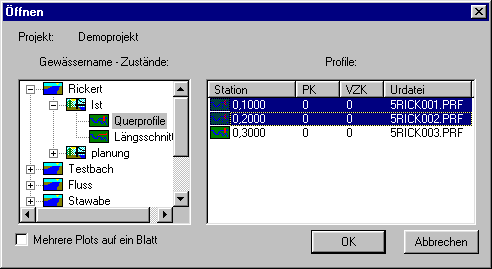
\includegraphics[scale=0.70]{projekt-oeffnen}
	\end{center}
	\caption{Projekt �ffnen}
	\label{fig:projekt-oeffnen}
\end{figure}
 

\hypertarget{cmd:datei-oeffen}{}
\hypertarget{dlg:profil-oeffnen}{}
\subsection{Profildaten einladen}
 
Nachdem ein Projekt ge�ffnet wurde, erscheint eine Baumstruktur, aus der zun�chst ein Gew�sser, dann ein Zustand und schlie�lich die Quer- oder L�ngsprofile, die dargestellt werden sollen, zu selektieren sind. 
Wird eine Mehrfachauswahl getroffen, so werden entweder die ausgew�hlten Profile als einzelne Plots ge�ffnet oder alternativ (Kontrollk�stchen \ctrl{Mehrere Plots auf ein Blatt} ist aktiviert) alle Profile auf demselben Blatt angezeigt (siehe Abschnitt~\ref{sec:multiplot}).

\begin{figure}[hbtp]
	\begin{center}
		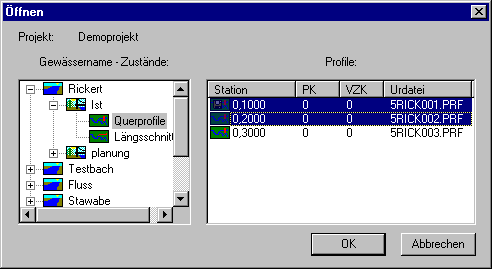
\includegraphics[scale=0.70]{offnen}
	\end{center}
	\caption{Auswahl darzustellender Profile im Verzeichnisbaum}
	\label{fig:auswahl-profile}
\end{figure}

Im Projektverzeichnis werden die Unterverzeichnisse \file{/plot\_ls} und \file{/plot\_qp} angelegt, in denen die 'Plotdateien' mit der Endung '\file{.wpl}' gespeichert werden. 

\hypertarget{cmd:projekt-schliessen}{}
Neben der Dateiauswahl im Verzeichnisbaum k�nnen die darzustellenden Profile auch unabh�ngig von der \wspwin-Projektverwaltung �ber ihren Dateinamen ge�ffnet werden. Hierzu ist im Plotter zun�chst das aktive Projekt zu schlie�en (Men� \menu{Datei / Projekt schliessen}) und anschlie�end eine Datei (\file{*.wpl} oder \file{*.prf}) auszuw�hlen (Men� \menu{Datei / �ffnen}). W�hrend bei ge�ffnetem Projekt unter dieser Option die Baumstruktur erscheint (Abb. \ref{fig:auswahl-profile}), sieht man bei geschlossenem Projekt ein Dateiauswahlfenster. 

\hypertarget{cmd:datei-einf�gen}{}
\subsection{Profildaten einf�gen}
�ber die Men�folge \menu{Datei / Daten Einf�gen} haben Sie die M�glichkeit
mehrere Profile inkl. aller Datens�tze wie Wasserspiegel und Sohlh�he zum Vergleich �bereinander zu
laden. W�hlen Sie das Vergleichsprofil aus und entscheiden Sie, ob es am
tiefsten Punkt des Ursprungsprofils ausgerichtet werden soll, oder ob es an einem bestimmten
Profilpunkt (Station) beginnen soll, der in dem entsprechenden Editierfeld einzugeben ist.

\hypertarget{cmd:datei-profiluebersicht}{}
Eine andere Form der Dateiauswahl ist �ber die Profil�bersicht (\menu{Datei / Profil�bersicht}) m�glich. Nach Wahl der Option erscheinen mehrere Profile (standardm��ig 6) gleichzeitig in einer �bersicht (Abb. \ref{fig:profiluebersicht}). Aus dieser �bersicht heraus k�nnen durch Doppelklick auf das entsprechende Profil Profile aufgerufen werden. 

\begin{figure}[hbtp]
	\begin{center}
		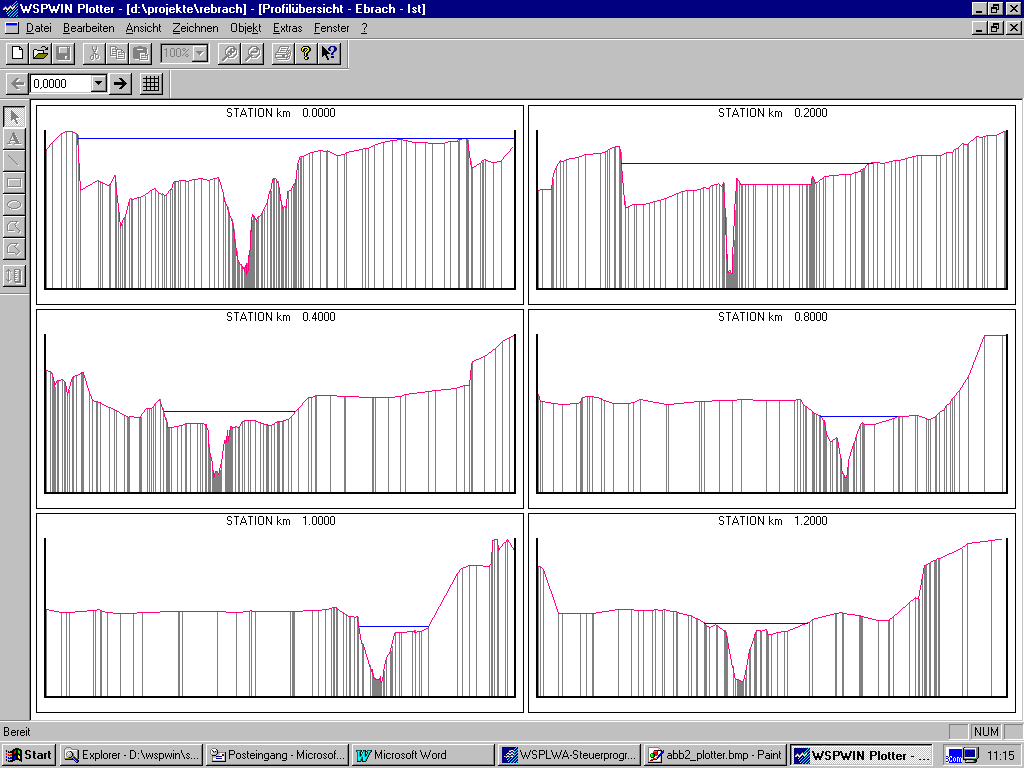
\includegraphics[scale=0.40]{profiluebersicht}
	\end{center}
	\caption{Profil�bersicht}
	\label{fig:profiluebersicht}
\end{figure}

\hypertarget{cmd:profiluebersicht-eigenschaften}{}
Die Anzahl der dargestellten Profile kann �ber das Nummernsymbol (Abb.~\ref{fig:profiluebersicht-props}) in der linken oberen Bildh�lfte eingestellt werden.

\begin{figure}[hbtp]
	\begin{center}
		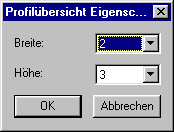
\includegraphics[scale=0.70]{profiluebersicht-props}
	\end{center}
	\caption{Einstellung der Eigenschaften der Profil�bersicht}
	\label{fig:profiluebersicht-props}
\end{figure}

Neben dem Nummernsymbol befindet sich ein Listenfeld mit einer Stationsangabe. Hier kann sowohl aus der Profil�bersicht heraus, wie auch aus der eigentlichen Plotansicht gezielt ein Profil �ber die Stationsangabe gew�hlt werden. Die Pfeile links und rechts hiervon erm�glichen es, auf die vorangehenden oder nachfolgenden Profile zu springen.


\hypertarget{cmd:bearbeiten-eigenschaften}{}
\section{Profildarstellung bearbeiten}
\label{sec:profildarstellung}

Sobald Sie eine Datei ausgew�hlt haben, wird automatisch ein vorformatierter Plot (vgl.
Abb. \ref{fig:formatierter-plot}) inklusive Stempel f�r Sie erzeugt. Er kann anschlie�end nach Ihren eigenen
W�nschen gestaltet werden. S�mtliche Formatierungsoptionen finden sich unter \menu{Bearbeiten / Eigenschaften}.

\begin{figure}[hbtp]
	\begin{center}
		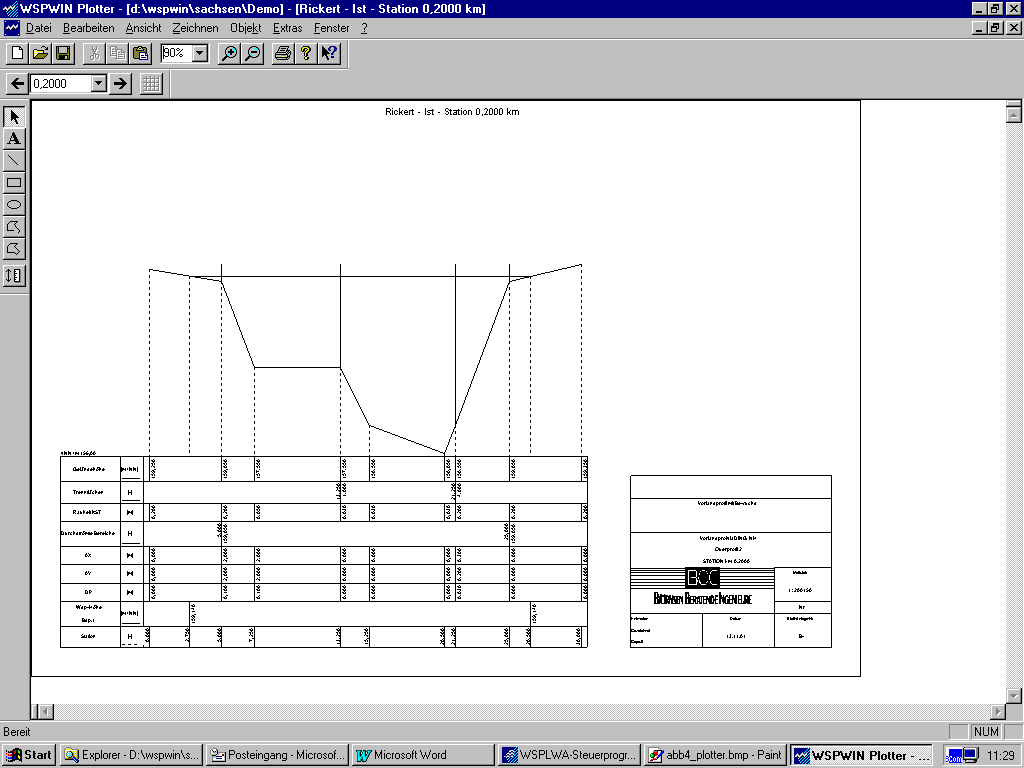
\includegraphics[scale=0.5]{formatierter-plot}
	\end{center}
	\caption{Standardformatierung eines Plots}
	\label{fig:formatierter-plot}
\end{figure}

Nachdem Sie die Men�folge \menu{Bearbeiten / Eigenschaften} gew�hlt haben, stehen
Ihnen in Form von Karteikarten eine Vielzahl von Formatierungsm�glichkeiten zur
Verf�gung (Abb. \ref{fig:dlg-eigenschaften}).

\begin{figure}[hbtp]
	\begin{center}
		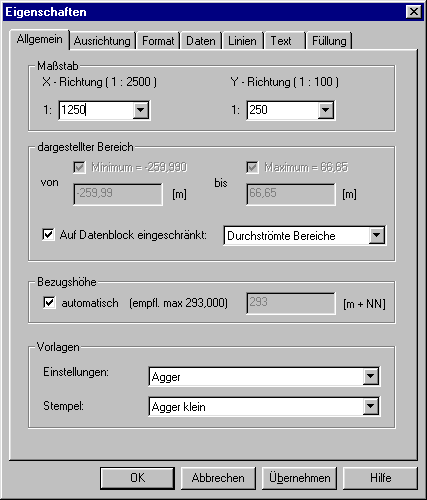
\includegraphics[scale=0.60]{dlg-eigenschaften}
	\end{center}
	\caption{Dialogfeld \dialog{Eigenschaften / Allgemein}}
	\label{fig:dlg-eigenschaften}
\end{figure}


\subsection{Allgemeine Eigenschaften}

\hypertarget{cmd:bearbeiten-eigenschaften-allgemein}{}
\hypertarget{dlg:bearbeiten-eigenschaften-allgemein}{}
�ber die erste Karteikarte \dialog{Allgemein} k�nnen folgende allgemeine Parameter modifiziert
werden:

\begin{itemize}
	\item{Ma�stab}\\
	\wspplot\ errechnet automatisch bezogen auf die eingestellte Papiergr��e einen x- und
	y-Ma�stab. Wenn die automatische Voreinstellung nicht �bernommen werden soll,
	k�nnen Sie die entsprechenden Listenfelder aufklappen und einen der hier angegebenen
	Ma�st�be selektieren oder direkt in die Editierfenster des Listenfeldes einen eigenen Wert
	eintragen. Soll sp�ter wieder auf die automatische Berechnung zur�ckgegriffen werden,
	ist die Einstellung '$<$automatisch$>$' aus dem Listenfeld zu selektieren. Der gerade
	eingestellte Ma�stab wird als Text �ber dem Listenfeld angezeigt. Bei der automatischen
	Berechnung werden nur Ma�st�be, die im Listenfeld aufgef�hrt sind, verwendet.
	
	\item{dargestellter Bereich}\\
	Es besteht die M�glichkeit den dargestellten Bereich eines Profils festzulegen. Zum einen 
	k�nnen manuell die Grenzen festgelegt werden, wobei die Ausma�e des Profils nicht �berschritten 
	werden d�rfen. Zm anderen kann die Darstellung durch Aktivierung des Kontrollk�stchens 'Auf Datenblock 
	eingeschr�nkt'  auf die Ausma�e eines bestimmten Datenblocks begrenzt werden. Wird also zum Beispiel der Datenblock 	  
	'Trennfl�chen' gew�hlt, so wird nur der Bereich innerhalb der Trennfl�chen dargestellt.
	Standardm��ig sind die Kontrollk�stchen 'Minimum' und 'Maximum' aktiviert, welche bewirken, da� der gesamte Profilbereich   angezeigt wird.
	
	\item{Bezugsh�he}\\
	Die Bezugsh�he errechnet sich automatisch in Abh�ngigkeit der Profildaten. Sollten Sie
	ein anderes Bezugsniveau f�r Ihre Profilzeichnung w�nschen, k�nnen Sie hier, nach
	Ausschalten des Kontrollk�stchens f�r die automatische �bernahme, einen Wert
	eingeben.

	\item {Einstellungen}\\
	Auf �hnliche Weise ist es m�glich, Formatvorlagen f�r die Plots zu erstellen und diese
	dem Plot zuzuordnen. �ber \menu{Einstellungen / Eigenschaften} k�nnen Sie die
	vorhandenen Standards (Erzeugung) aus\-w�h\-len und dem aktuellen Plot zuordnen.
	
	\item{Stempel}\\
	�ber den Stempeleditor ist es m�glich, einen individuellen Stempel zu kreieren.
	Jedem Stempel ist ein Name zuzuordnen, �ber den er an dieser Stelle angesprochen
	werden kann. Alle verf�gbaren Stempel werden hier aufgef�hrt und es kann aus dem
	entsprechenden Listenfeld der dem jeweiligen Plot zuzuordnende Stempel ausgew�hlt
	werden.
	
\end{itemize}


\subsection{Abst�nde und Ausrichtung der Zeichenelemente}

\hypertarget{dlg:bearbeiten-eigenschaften-ausrichtung}{}
�ber die Karteikarte \dialog{Ausrichtung} lassen sich Abst�nde und Ausrichtung von Profil und Stempel einstellen (Abb. \ref{fig:dlg-eigenschaften-ausrichtung})

\begin{figure}[hbtp]
	\begin{center}
		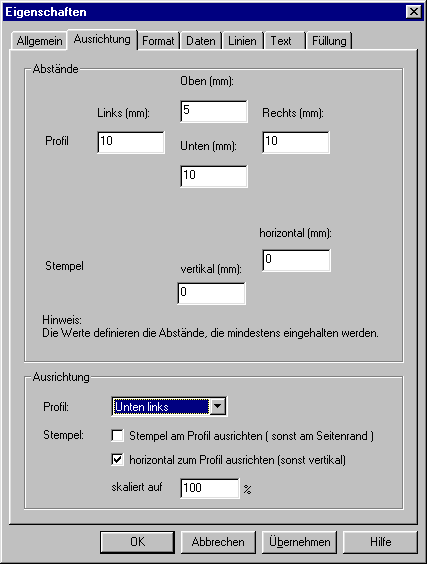
\includegraphics[width=0.8\linewidth]{dlg-eigenschaften-ausrichtung}
	\end{center}
	\caption{Dialogfeld \dialog{Eigenschaften / Ausrichtung}}
	\label{fig:dlg-eigenschaften-ausrichtung}
\end{figure}

In der oberen Dialogh�lfte (\ctrl{Abst�nde}) lassen sich die Abst�nde zum Profil (d.h. Profil und Tabelle) und zum Stempel einstellen. 
Alle Abst�nde bezeichnen dabei die Mindestabst�nde, die entweder zum Rand oder zum jeweils anderen Zeichnungselement (d.h. Profil zum Stempel oder umgekehrt) eingehalten werden.

In der unteren Dialogh�lfte (\ctrl{Ausrichtung}) kann der Benutzer einstellen, in welche Richtung das Profil ausgerichtet werden soll. Zur Zeit stehen die Richtungen 'Unten links', 'Unten rechts', 'Oben links' und 'Oben rechts' zur Verf�gung.

Der Stempel wird dann je nach Einstellung horizontal oder vertikal neben dem Profil angeordnet. Weiterhin l�sst sich einstellen, ob der Stempel dabei m�glichst entfernt vom Profil (am Seitenrand ausrichten) oder m�glichst nah am Profil (am Profil ausrichten) angeordnet wird.

Schlie�lich kann f�r den Stempel eine Skalierung eingestellt werden. Es sind Werte zwischen 10 und 1000\% m�glich.

\subsection{Format}

\hypertarget{dlg:bearbeiten-eigenschaften-format}{}
Weitere M�glichkeiten zur �nderungen der Darstellungen von Profil und Tabelle bietet die Karteikarte \dialog{Format} (Abb. \ref{fig:dlg-eigenschaften-format}).

\begin{figure}[hbtp]
	\begin{center}
		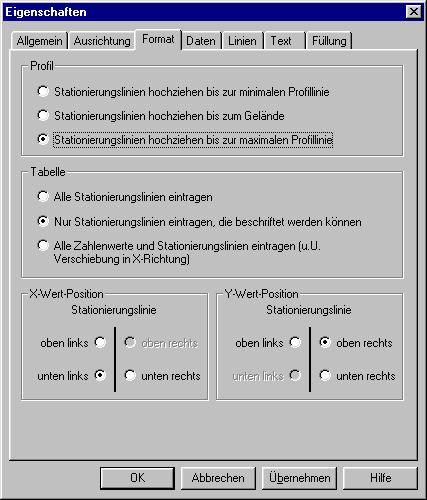
\includegraphics[scale=0.60]{dlg-eigenschaften-format}
	\end{center}
	\caption{Dialogfeld \dialog{Eigenschaften / Format}}
	\label{fig:dlg-eigenschaften-format}
\end{figure}

Die Einstellungsm�glichkeiten im Einzelnen:

\begin{itemize}

\item{Profil}\\
Hier kann eingestellt werden, bis wohin die senkrechten Stationierungslinien im Profil gezogen werden. Es kann bis zum Minimum oder zum Maximum aller dargestellten Datens�tze gezeichnet werden ('Stationierungslinien hochziehen bis zur minimalen Profillinie' oder 'Stationierungslinien hochziehen bis zur maximalen Profillinie'), oder stets bis zur Gel�ndeh�he ('Stationierungslinien hochziehen bis zum Gel�nde').

\item{Tabelle}\\
Im Unterpunkt 'Tabelle' hat der Benutzer die M�glichkeit zu entscheiden, welche Stationierungslinien in die Tabelle eingetragen werden.

\item{X-Wert Position / Y-Wert Position}\\
Durch diese beiden Punkte wird die Ausrichtung der Beschriftung von X- und Y-Werten in der Tabelle bestimmt. M�glich sind hierbei die Positionen 'Oben links', 'Oben rechts', 'Unten links' und 'Unten rechts'. X- und Y-Wert k�nnen hierbei aber nie die gleiche Position einnehmen.

\end{itemize}


\subsection{Selektion der darzustellenden Datens�tze}
\label{sec:profildarstellung:daten}

\hypertarget{dlg:bearbeiten-eigenschaften-daten}
Der f�r Sie vorformatierte Plot enth�lt automatisch eine Vielzahl von Datens�tzen.
Normalerweise wird man zuerst einmal entscheiden, welche Datens�tze im Schriftfeld und
welche in der Zeichnung selbst mit aufgenommen werden sollen. Dies erfolgt �ber das Dialogfeld \dialog{Eigenschaften / Daten} (Abb. \ref{fig:dlg-eigenschaften-daten}).

\begin{figure}[hbtp]
	\begin{center}
		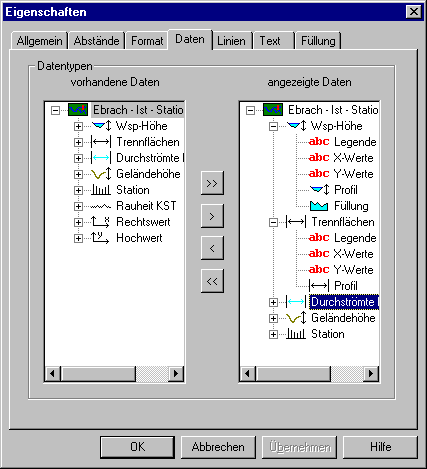
\includegraphics[scale=0.60]{dlg-eigenschaften-daten}
	\end{center}
	\caption{Dialogfeld \dialog{Eigenschaften / Daten}}
	\label{fig:dlg-eigenschaften-daten}
\end{figure}

Sobald Sie auf das K�stchen vor dem Gew�ssernamen klicken, werden Ihnen links alle im
Profil vorhandenen Datens�tze und rechts alle im Profil dargestellten Parameter angezeigt.
Wenn Sie einen Datensatz markieren und auf die Pfeiltasten in der Bildmitte klicken, k�nnen
Sie den Datensatz zu den angezeigten Daten hinzuf�gen oder entfernen. Sobald Sie einen
Datensatz �ber das Kreuz davor aufklappen, k�nnen Sie auf gleiche Weise die Form der
Darstellung ausw�hlen. Folgende Wahlm�glichkeiten stehen zur Verf�gung:

\begin{itemize}
	\item{Legende:} Der Datensatzname wird im Schriftfeld links namentlich mit aufgef�hrt
	\item{Profil:} Der Datensatz wird gezeichnet
	\item{X-Werte:} Die y-Werte werden im Schriftfeld mit aufgef�hrt
	\item{Y-Werte:} Die z-Werte werden im Schriftfeld mit aufgef�hrt
	\item{F�llung (nicht bei allen Datens�tzen verf�gbar):} Der Datensatz wird fl�chig gezeichnet
\end{itemize}

Sobald Sie OK (Dialog schlie�t sich) oder \menu{�bernehmen} (Dialog bleibt offen) w�hlen,
wird die Auswahl �bernommen.

\subsection{Linien und F�llungen}

\hypertarget{dlg:bearbeiten-eigenschaften-linien}{}
\hypertarget{dlg:bearbeiten-eigenschaften-fuellungen}{}
F�r die in die Zeichnung aufgenommen Datens�tze (siehe Absatz \ref{sec:profildarstellung:daten}) stehen 
verschiedene Formatierungsm�glichkeiten zur Verf�gung.
�ber die Karteikarte \dialog{Linien} k�nnen Sie Linientyp, -breite und -farbe
f�r Tabelle, Stempel und Rahmen ausw�hlen. Sobald Sie das K�stchen vor dem
Gew�ssernamen aufklappen (Abb. \ref{fig:dlg-eigenschaften-linien}), k�nnen Sie f�r jeden gezeichneten Datensatz diese
Optionen bestimmen.

\begin{figure}[hbtp]
	\begin{center}
		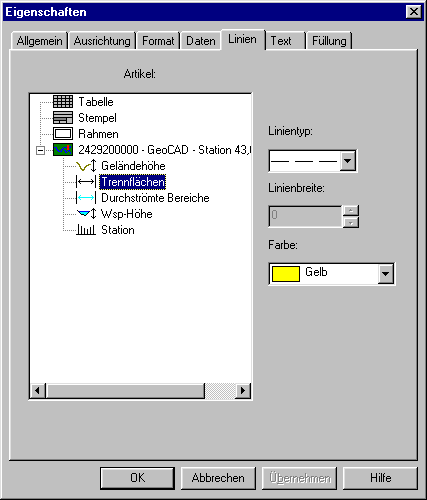
\includegraphics[scale=0.60]{dlg-eigenschaften-linien}
	\end{center}
	\caption{Dialogfeld \dialog{Eigenschaften / Linien}}
	\label{fig:dlg-eigenschaften-linien}
\end{figure}

F�r die Datens�tze, die �ber die Karteikarte \dialog{Daten}, mit F�llungen versehen wurden, kann
 mit der Karteikarte \dialog{F�llungen} die Art der F�llung festgelegt
werden. Zun�chst ist das Kontrollk�stchen \ctrl{Gef�llt} zu aktivieren, danach k�nnen f�r die
markierten Datens�tze Farbe und Muster der F�llung �ber die Listenfelder festgelegt werden.
Linienart und F�llung k�nnen auch interaktiv in der Karte ver�ndert werden. Klicken Sie
doppelt auf die zu formatierende Linie oder Fl�che. Es erscheint ein Dialogfenster, das Ihnen
die Formatierungseinstellungen f�r Linien und Fl�chen erm�glicht. Diese Option kann auch
nach dem Markieren durch \key{Rechte Maustaste} und \menu{Attribute} verf�gbar gemacht
werden.

\subsection{Textformatierungen}

\hypertarget{dlg:bearbeiten-eigenschaften-text}
�ber \menu{Bearbeiten / Eigenschaften / Text} k�nnen fast alle Texte des Plots eingegeben
und formatiert werden (Abb. \ref{fig:dlg-eigenschaften-text}).

\begin{figure}[hbtp]
	\begin{center}
		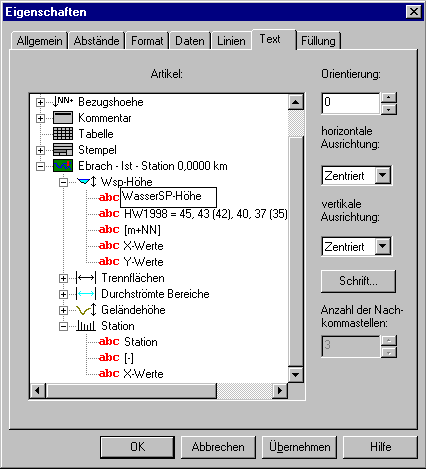
\includegraphics[scale=0.60]{dlg-eigenschaften-text}
	\end{center}
	\caption{Dialogfeld \dialog{Eigenschaften / Text}}
	\label{fig:dlg-eigenschaften-text}
\end{figure}

Folgende Texte werden unterschieden, die Sie durch Klicken des Kreuzes davor aufklappen
k�nnen. An den mit '\emph{abc}' rot markierten Stellen k�nnen Sie (au�er bei x- und y-Werten) durch
Markieren und explizites Klicken in das Feld einen beliebigen Text eingeben.

\begin{itemize}
	\item{Titel:} In die Zeichnungs�berschrift werden standardm��ig der Ge\-w�sser\-name, der Zustand und
		die Stationsangabe �ber Platzhalter eingetragen. Diese k�nnen bei Bedarf gel�scht und
		durch einen beliebigen Text �berschrieben werden.
	\item{Bezugsh�he:} Der Wert der Bezugsh�he wird automatisch auch �ber Platzhalter links zwischen
		Schriftfeld und Tabelle angegeben. Auch hier kann ein beliebiger Text eingegeben werden
		(z.B. HN statt NN).
	\item{Kommentar:} Der im Querprofil in \wspwin\ eingetragene Kommentar wird hier �ber den
		Platzhalter 'Comment' angezeigt.
	\item{Tabelle:} F�r das gesamte Schriftfeld kann die Schriftgr��e und die Anzahl
		Nachkommastellen festgelegt werden.
	\item{Stempel:} Im Stempeleditor k�nnen verschiedene Platzhalter (z.B. Auftraggeber, Datum,
		Blattnummer, �berschrift...) vergeben werden, f�r die an dieser Stelle, wiederum durch
		Anklicken des abc-Editierfeldes, Text eingegeben und formatiert werden kann.
	\item{Gew�sser / Zustand (Datens�tze):} Schlie�lich k�nnen durch Aufklappen der einzelnen
		Datens�tze, Texteingaben und Formatierungen f�r die Datensatzbezeichnung und die
		Dimension, sowie die Schriftart und Anzahl Nachkommastellen der y- und z-Werte
		eingegeben werden.
\end{itemize}

S�mtliche Textformatierungen k�nnen ebenfalls interaktiv durch Markieren eines Textes in
der Graphik und Doppelklick bzw. rechte Maus und Attribute vorgenommen werden.
\section{Zeichnung bearbeiten}

Neben den Einstellungsm�glichkeiten, welche das Dialogfeld \menu{Bearbeiten / Eigenschaften} bietet, kann die Zeichnung durch den Benutzer auch direkt manipuliert werden. Unter anderem besteht die M�glichkeit benutzerdefinierte Objekte einzuf�gen und zu ver�ndern oder Elemente des Profildarstellung direkt zu �ndern oder zu l�schen.

\hypertarget{cmd:zeichnen-select}{}
\hypertarget{cmd:zeichnen-text}{}
\hypertarget{cmd:zeichnen-linie}{}
\hypertarget{cmd:zeichnen-rechteck}{}
\hypertarget{cmd:zeichnen-ellipse}{}
\hypertarget{cmd:zeichnen-linienzug}{}
\hypertarget{cmd:zeichnen-vieleck}{}
\hypertarget{toolbar:draw}{}
\subsection{Benutzerdefinierte Objekte erstellen}

�ber die Zeichensymbolleiste an der linken Bildseite (Abb. \ref{fig:toolbar-draw}) k�nnen Sie in die Graphik auch eigene
Texte und Zeichnungen einf�gen.

\begin{figure}[hbtp]
	\begin{center}
		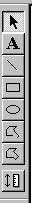
\includegraphics[scale=0.80]{toolbar-draw}
	\end{center}
	\caption{Zeichensymbolleiste}
	\label{fig:toolbar-draw}
\end{figure}

Wenn Sie einen Text einf�gen m�chten, w�hlen Sie das \textbf{A},
so da� Sie sich im Textmodus befinden. Dann ziehen Sie in der Graphik an der gew�nschten
Stelle ein Textfeld bei gedr�ckter linker Maustaste auf. Sobald Sie die Maus loslassen, blinkt
ein Cursorzeichen und Sie k�nnen mit der Texteingabe beginnen. Der jeweilige
Bearbeitungsmodus wird durch Klicken auf die Pfeiltaste der Zeichensymbolleiste beendet.
Sie k�nnen einen Text jederzeit wieder modifizieren, wenn Sie das Textobjekt markieren und
das \textbf{A} aktivieren. Die �brigen Zeichenmodi sind wie in entsprechenden Zeichenprogrammen
zu handhaben. 

\hypertarget{cmd:zeichnen-messen}
�ber das Linealsymbol k�nnen Strecken gemessen werden, in dem Sie auf das
Symbol klicken und bei gedr�ckter linker Maustaste eine Linie nachzeichnen. Es erscheint der
berechnete Abstand.

\hypertarget{cmd:objekt-einfuegen}
Zus�tzlich zur Zeichensymbolleiste k�nnen Sie �ber \menu{Bearbeiten / Neues Objekt einf�gen} auch bereits gespeicherte Objekte (z.B. Bilddateien) einf�gen bzw. auf
Programme mit OLE-Schnittstelle zugreifen und hier Objekte erstellen, die Sie direkt in ihren
Plot einbinden k�nnen (Abb. \ref{fig:objekt-einfuegen}).

\begin{figure}[hbtb]
	\begin{center}
		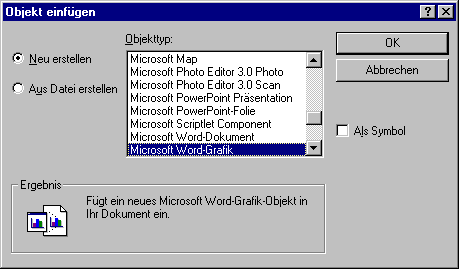
\includegraphics[scale=0.80]{objekt-einfuegen}
	\end{center}
	\caption{Objekt einf�gen}
	\label{fig:objekt-einfuegen}
\end{figure}


%cmd:bearbeiten-rueckgaengig
%cmd:bearbeiten-ausschneiden
\hypertarget{cmd:bearbeiten-ausschneiden}{}
\hypertarget{cmd:bearbeiten-kopieren}{}
\hypertarget{cmd:bearbeiten-einf�gen}{}
\hypertarget{cmd:bearbeiten-loeschen}{}
\hypertarget{cmd:bearbeiten-inhalte-einfuegen}{}
\hypertarget{cmd:objekt-z-order}{}
\hypertarget{cmd:objekt-attribute}{}
\wspplot bietet eine Menge an M�glichkeiten sowohl benutzerdefinierte als auch automatisch erstellte Objekte zu manipulieren.

So lassen sich alle benutzerdefinierten Objekte, sowie die Zeichnungs\-�ber\-schrift, der Kommentar und die Bezugsh�he nach Selektion mit der Maus verschieben. Benutzerdefinierte Objekte k�nnen dar�berhinaus in Ihrer Gr�sse bzw. Form ( z.B. im Falle von Linienz�gen ) ver�ndert werden. 

\subsection{Objekte bearbeiten}

Um die Attribute wie z.B. Farbe, Schriftart o. �. eines Objektes zu �ndern, kann der Dialog \dialog{Attribute} durch Doppelklick auf ein Objekt aktiviert werden. Dieser Dialog ist auch �ber den Men�punkt \menu{Objekt / Attribute} oder �ber das Kontextmen� der rechten Maustaste zug�nglich.

Da sich Objekte gegenseitig �berdecken k�nnen, kann die Lage jedes Objektes in der Zeichenebene durch die Unterpunkte \menu{Nach oben setzen}, \menu{Nach unten setzen}, \menu{Eins nach oben setzen} und \menu{Eins nach unten setzen} des Men�punktes \menu{Objekt} ver�ndert werden. Dies ist insbesondere dann notwendig, wenn sich ein Objekt nicht selektieren l�sst, da es durch ein dar�berliegendes verdeckt wird.

�ber die Unterpunkte \menu{Ausschneiden}, \menu{Kopieren} und \menu{Einf�gen} des Men�punkts \menu{Bearbeiten}, lassen sich beliebige Objekte ausschneiden, kopieren und wieder einf�gen.

Bis auf die Umrandung der Tabelle und den Tabellenschl�ssel lassen sich alle Objekte durch den Men�punkt \menu{Bearbeiten / L�schen} bzw. einen Druck auf die \key{Entf}-Taste aus der Zeichnung nehmen. Da sich bei Objekten aus dem Stempel oder dem Profil die Ausmasse der Zeichnung �ndern k�nnte, muss in diesem Fall die Zeichnung neu formatiert werden.
Wurden Objekte aus dem Profil oder der Tabelle entfernt, so lassen sich diese durch ein erneutes Einf�gen des entsprechenden Datensatzes im Dialog \dialog{Eigenschaften / Daten} wiederherstellen.


\hypertarget{cdm:objekt-fixieren}{}
\subsection{Objekte am Profil fixieren}

Bei benutzerdefinierten Objekten besteht weiterhin �ber den Men�punkt \menu{Objekt / Am Profil fixiert} die M�glichkeit diese am Profil zu fixieren. Dazu sollte das Objekt sich vollst�ndig innerhalb des Profils befinden, da sich sonst die Ausmasse der Zeichnung ver�ndern k�nnten. Ist ein Objekt am Profil fixiert, so beh�lt es seine relative Position innerhalb des Profils stets bei und wird nicht z.B. durch eine �nderung des Ma�stabs verschoben.
\hypertarget{cmd:multiplot}{}
\section{Mehrere Plots auf ein Blatt}
\label{sec:multiplot}

Wird beim Laden der Profildaten die Option \ctrl{Mehrere Plots auf ein Blatt} selektiert (siehe Abbildung~\ref{fig:auswahl-profile}), so werden alle ausgew�hlten Profile in einem Plotter-Fenster ge�ffnet. Die Profile werden dabei mit der vorgegebenen Standardvorlage (siehe Abschnitt~\ref{sec:templates}) formatiert und Zeilenweise angeordnet. Ist in der Standardvorlage ein Stempel ausgew�hlt, so wird dieser rechts unten plaziert.

\begin{figure}[htbp]
	\centering
	% FEHLT!
	%\includegraphics[width=1.0\textwidth]{multiplot} 
	\caption{Mehrere Plots auf einem Blatt}
	\label{fig:multiplot}
\end{figure}

Passen nicht alle Profile auf ein einzelnes Blatt (zum Einstellen der Seitengr�sse siehe Abschnitt~\ref{sec:print_plot}), so werden wie im Plotter �blich mehrere Bl�tter erstellt und die Blattgrenzen durch blaue Linien dargestellt. Passt ein Profil nicht vollst�ndig auf ein Blatt, so wird es komplett weggelassen und eine entsprechende Meldung ausgegeben.

Prinzipiell stehen im Modus 'mehrere Plots auf ein Blatt' die gleichen Bearbeitungsm�glichkeiten zur Verf�gung wie im normalen Modus. Lediglich die Profildarstellung wird ausschliesslich �ber die Standardvorlage gesteuert und kann nachtr�glich nicht mehr ver�ndert werden. Statt dem entsprechenden Dialog im Einzelprofilmodus steht durch das Men� \menu{Bearbeiten / Eigenschaften} ein Dialog zum Einstellen der Abst�nde zwischen den Profilen und zum �ndern der Blatt�berschrift zur Verf�gung.

\begin{figure}[htbp]
	\centering
	% FEHLT
	%\includegraphics[width=0.6\textwidth]{multiplot_props}
	\caption{Einstellungen f�r 'Mehrere Plots auf ein Blatt'}
	\label{fig:multiplot_properties}
\end{figure}
\hypertarget{cmd:extras-stempel}{}
\section{Stempeleditor}

\wspplot\ bietet Ihnen die M�glichkeit, neben dem \bce-Stempel auch eigene
Stempel mit ihrem Firmen- / Institutslogo bzw -layout zu integrieren. Hierzu steht ein
eigenst�ndiges Programm, der Stempeleditor, zur Verf�gung, den Sie �ber \menu{Extras / Stempeleditor}
aus dem Plotterprogramm heraus aufrufen k�nnen. Standardm��ig wird
Ihnen ein Stempel, entweder der BCE-Stempel oder der Stempel des Bayerischen
Landesamtes f�r Wasserwirtschaft mitgeliefert. Der mitgelieferte Stempel findet sich im
Plotterinstallationsverzeichnis (standardm��ig \file{C:/Programm/BCE/Wspwin/Plotter}) und hat die Endung '\file{.stp}'. Ein vorhandener Stempel kann �ber \menu{Datei / �ffnen} im Stempeleditor
ausgew�hlt werden. W�hlen Sie \menu{Datei / Neu}, wenn Sie einen neuen Stempel erzeugen
m�chten. Es sind dann zun�chst die Eigenschaften des Stempels, d.h. seine Gr��e und der
Name, �ber den der Stempel aus dem eigentlichen Plotprogramm heraus aufgerufen wird,
anzugeben (Abb. \ref{fig:stempel-eigenschaften}).

\begin{figure}[hbtp]
	\begin{center}
		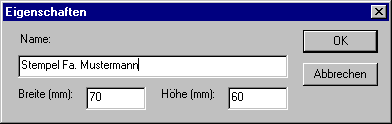
\includegraphics[scale=0.80]{stempel-eigenschaften}
	\end{center}
	\caption{Stempeleigenschaften}
	\label{fig:stempel-eigenschaften}
\end{figure}

Zur Generierung des Stempels steht eine Zeichensymbolleiste wie im eigentlichen
Plotterprogramm zur Verf�gung. Die Funktionen stehen auch im Men�punkt \menu{Zeichnen} zur
Verf�gung. Texte k�nnen nach Anklicken des A-Symbols und Aufziehen eines Textfeldes
eingegeben werden. Standardm��ig wird das Textfeld mit einem Platzhalter (z.B.
Auftraggeber) vorbesetzt. Wenn man in dem Feld einen Doppelklick ausf�hrt, gelangt man
wieder in die Attributmaske (vgl. Abb. \ref{fig:stempel-attribute}). 
In dem Listenfeld \ctrl{Typ} finden sich eine Vielzahl
von Platzhaltern, von denen man den gew�nschten selektieren kann. M�chte man keinen
Platzhalter verwenden, w�hlt man in dem Listenfeld '$<$keine$>$'. In diesem Fall kann man unter
\ctrl{Text} in dem Dialogfenster \dialog{Graphische Attribute} direkt einen beliebigen Text
eingeben. Alternativ kann man auch das Textfeld im Stempel markieren und nach Wahl des
A-Symbols in dem Feld selbst editieren. Hilfreich bei der Erstellung eines neuen Stempels
kann eine Gittereinrichtung sein. Die Gittergr��e legen Sie unter \menu{Extras / Gittereinrichtung}
fest (Abb. \ref{fig:stempel-gitter}). Hier bestimmen Sie auch �ber das Kontrollk�stchen
'An Gitter ausrichten', ob neu erstellte Objekte (Texte oder Zeichnungen) automatisch
am Gitternetz �ber einen Objektfang ausgerichtet werden sollen und so symmetrisch plaziert
werden.
�ber \menu{Bearbeiten / Neues Objekt einf�gen} k�nnen Sie wie im Plotter selbst fertige
Bilddateien einf�gen oder auf Programme mit OLE-Funktion zugreifen, Objekte erstellen und
diese in den Stempel integrieren. Auf diese Weise k�nnen Sie z.B ihr Firmenlogo integrieren.
F�r den Plotter wie auch den Stempeleditor ist zu beachten, da� s�mtliche Objekte wie Layer
aufzufassen sind, d.h. es kann vorkommen, da� das eine Objekt das andere �berdeckt. In
diesem Fall k�nnen Sie nach Markieren eines Objektes �ber \menu{Objekt / nach oben / unten setzen}
die Hierarchie der Darstellung modifizieren. Dies ist auch bei der
Darstellung verschiedener Datens�tze (z.B. fl�chige Darstellung mehrerer Wasserspiegel) im
Plotter zu beachten.

\begin{figure}[hbtp]
	\begin{center}
		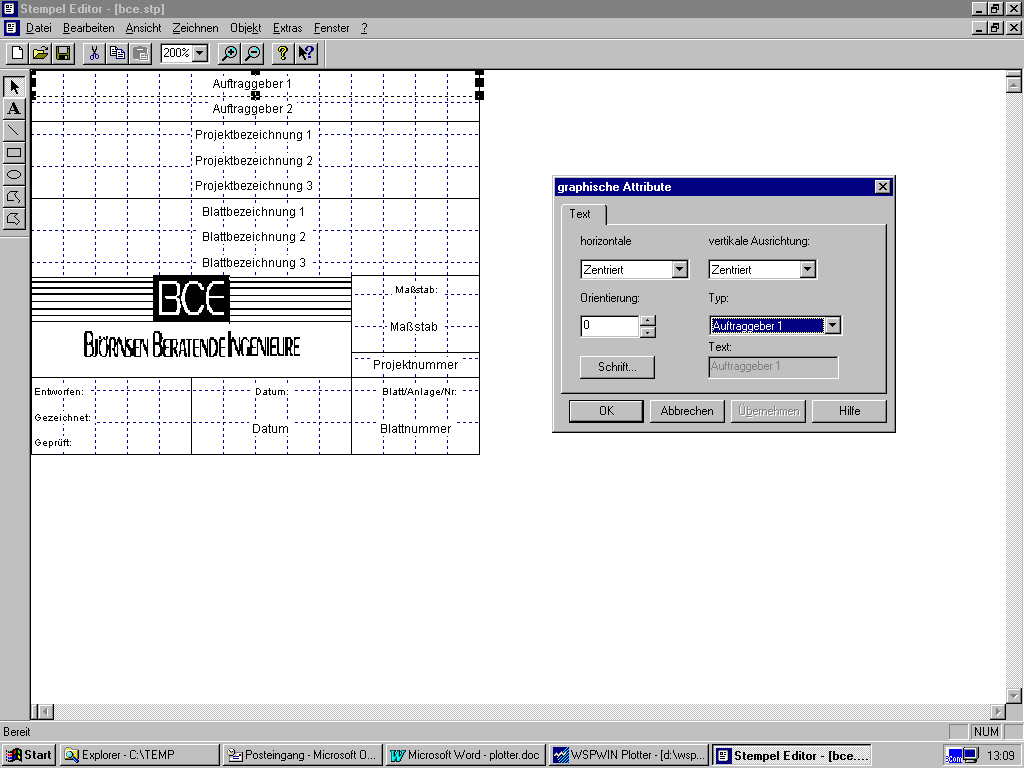
\includegraphics[scale=0.40]{stempel-attribute}
	\end{center}
	\caption{\bce-Stempel und graphische Attribute eines Textfeldes im Stempeleditor}
	\label{fig:stempel-attribute}
\end{figure}

\begin{figure}[hbtp]
	\begin{center}
		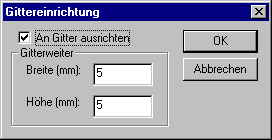
\includegraphics[scale=0.80]{stempel-gitter}
	\end{center}
	\caption{BCE-Stempel und graphische Attribute eines Textfeldes im Stempeleditor}
	\label{fig:stempel-gitter}
\end{figure}

\hypertarget{cmd:extras-standard}{}
\section{Standardlayouts erstellen und bearbeiten}
\label{sec:templates}
Um nicht jeden Plot einzeln formatieren zu m�ssen, k�nnen auch Standardlayouts erstellt
werden, die dann relativ einfach auf neue Plots �bertragen werden k�nnen. W�hlen Sie hierzu
\menu{Extras / Standard} (Abb. \ref{fig:standardeinstellungen}).
Wenn Sie einen neuen Standard erzeugen m�chten, w�hlen Sie \ctrl{Hinzuf�gen}. Es
erscheinen zwei Editierfelder, in denen Sie zum einen nach Klicken in das Einstellungen-Feld
(links) einen Namen f�r Ihr Layout vergeben k�nnen (z.B. LfW-Querprofil) und zum anderen
einen Stempel zuordnen k�nnen. Sobald Sie in das Stempelfeld klicken erscheint ein
Listenfeld mit allen verf�gbaren Stempeln. Wenn Sie eine Standardeinstellung markieren und
anschlie�end \ctrl{Bearbeiten} dr�cken, kommen Sie wieder zum Dialogfeld \dialog{Eigenschaften}.
Hier k�nnen Sie s�mtliche Einstellungen wie unter \ref{sec:profildarstellung}
erl�utert selektieren und dem Standard zuordnen. Beim sp�teren �ffnen eines neuen
Plots / Profils wird als Default der Standard gew�hlt, dessen Kontrollk�stchen aktiv geschaltet
wurde. Es besteht auch die M�glichkeit keinen Standard vorzudefinieren (alle K�stchen
ausgeschaltet). Um einem einzelnen Plot einen Standard zuzuordnen w�hlen Sie in der Karte
\dialog{Allgemein} unter \ctrl{Einstellungen / Eigenschaften} das gew�nschte Layout aus.

\begin{figure}[h]
	\begin{center}
		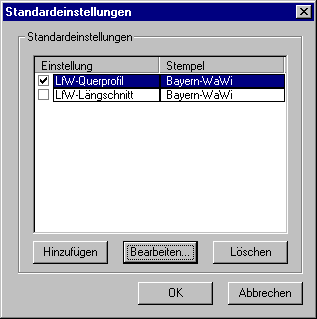
\includegraphics[scale=0.80]{standardeinstellungen}
	\end{center}
	\caption{Standardeinstellungen}
	\label{fig:standardeinstellungen}
\end{figure}

\hypertarget{cmd:seite-einrichten}{}
\hypertarget{cmd:druck-vorschau}{}
\hypertarget{cmd:drucken}{}
\hypertarget{cmd:drucken-alles}{}
\hypertarget{cmd:drucker-einrichten}{}
\section{Drucken / Plotten}
\label{sec:print_plot}
Bevor Sie die Zeichnung zum Drucker bzw. Plotter schicken, haben Sie noch weitere
M�glichkeiten, die Seite einzurichten.
Innerhalb einer Arbeitssitzung mit \wspplot\ k�nnen Sie eine Standard Seiten-
/Druckereinrichtung �ber \menu{Datei / Druckereinrichtung (Standard) } festlegen (Abb. \ref{fig:seite-einrichten}).
Hier w�hlen Sie den zu verwendenden Drucker sowie die Papiergr��e aus und legen die
R�nder (Abstand Papierrand-Rahmen) fest. Nachdem Sie die Standarddruckereinrichtung
festgelegt haben, werden alle Profile, die Sie danach �ffnen, automatisch mit dieser
Standarddruckereinrichtung formatiert. Genau die gleichen Einstellungen lassen sich unter
\menu{Datei / Seite einrichten} f�r einen Einzelplot festlegen. Die Standardeinstellungen
bleiben nur so lange g�ltig, wie das Programm nicht wieder geschlossen wird.

\begin{figure}[hbtp]
	\begin{center}
		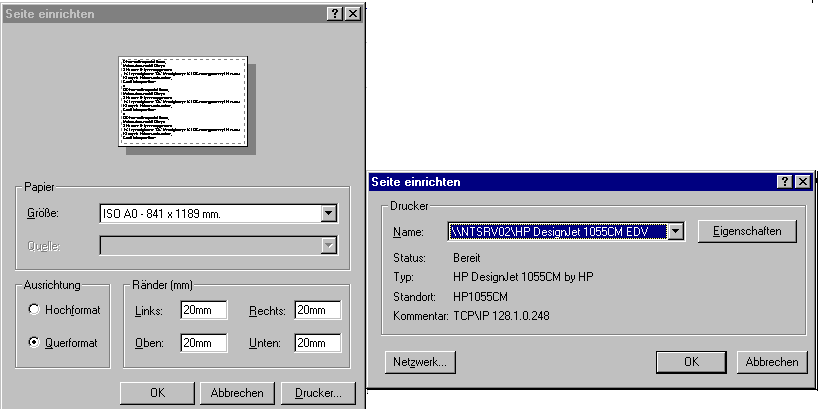
\includegraphics[scale=0.70]{seite-einrichten}
	\end{center}
	\caption{Seite einrichten}
	\label{fig:seite-einrichten}
\end{figure}

�ber \menu{Datei / Drucken} schicken Sie den Plot zu ihrem Ausgabeger�t.

\hypertarget{cmd:datei-speichern}{}
\hypertarget{cmd:datei-speichern-unter}{}
\section{Zeichnungen speichern und exportieren}

Die Plots k�nnen jederzeit �ber \menu{Datei / speichern} gesichert werden. Die Namensvergabe erfolgt dann automatisch. �ber \menu{Datei-speichern unter} haben Sie die M�glichkeit, selbst einen Dateinamen zu vergeben. So k�nnen Sie z.B. auch mehrere unterschiedliche Plots f�r eine Profildatei anlegen, die Sie dann auf die soeben beschriebene Weise (nach vorherigem \menu{Projekt-schliessen} ) wieder �ffnen k�nnen.
Es ist zu empfehlen, die Plots h�ufiger zwischendurch zu speichern, damit aufwendige Formatierungen nicht Gefahr laufen, verloren zu gehen. 

\hypertarget{cmd:datei-dxf-export}{}
Alternativ k�nnen Sie �ber \menu{Datei / Dxf Export} eine dxf-Datei erstellen, die Sie in einem CAD-Programm
einlesen und ggf. weiter aufbereiten k�nnen.

\listoffigures
\clearpage

%\listoftables
%\clearpage

%\printindex

\end{document}
